\documentclass[12pt, titlepage]{article}
\usepackage[shortlabels]{enumitem}
\usepackage{booktabs}
\usepackage{tabularx}
\usepackage{hyperref}
\usepackage{graphicx}
\usepackage{mdframed}
\usepackage{float}
\hypersetup{
    colorlinks,
    citecolor=black,
    filecolor=black,
    linkcolor=red,
    urlcolor=blue
}
\usepackage[round]{natbib}

\title{SE 3XA3: Test Report\\GoDBMS}

\author{Team \#7, Databased
		\\ Faiq Ahmed, ahmedf46
		\\ Eesha Qureshi, qureshe
		\\ Kevin Kannammalil, kannammk
}

\date{April 12th, 2022}

\begin{document}

\maketitle

\pagenumbering{roman}
\tableofcontents
\listoftables
\listoffigures

\begin{table}[H]
\caption{\bf Revision History}
\begin{tabularx}{\textwidth}{p{3cm}p{2cm}X}
\toprule {\bf Date} & {\bf Version} & {\bf Notes}\\
\midrule
April 11, 2022 & 1.0 & Initial Document \\
April 11, 2022 & 1.2 & Started Test Cases \\
April 12, 2022 & 1.2 & Finished Test Cases \\
April 12, 2022 & 1.2 & Completed Document \\
\bottomrule
\end{tabularx}
\end{table}

\newpage

\pagenumbering{arabic}

% \section{General Information}

% \subsection{Purpose}
The purpose of this document is to provide the outcome of the testing methods that were laid out in the Test Plan document. This document includes the assessment of how successful the Functional and Non Functional requirements that were created during the development process and the traceability of those requirements throughout the process.

% \subsection{Acronyms, Abbreviations, and Symbols}
	
\begin{table}[H]
\caption{\textbf{Table of Abbreviations}} \label{Table}

\begin{tabularx}{\textwidth}{p{3cm}X}
\toprule
\textbf{Abbreviation} & \textbf{Definition} \\
\midrule
SRS & Software Requirements Specification; a document that outlines important information about the software project such as stakeholders, functional requirements, non-functional requirements and project scope \\
POC & Proof of Concept; a prototype, demo or design that provides evidence of the project's feasibility \\
DBMS & \textbf{Database} Management System; software that allows a user to perform \textbf{database} transactions and operations\\
CLI & Command Line Interface; the point of communication between the software and the user \\
Go & GoLang \\
\bottomrule
\end{tabularx}

\end{table}

\begin{table}[H]
\caption{\textbf{Table of Definitions}} \label{Table}

\begin{tabularx}{\textwidth}{p{3cm}X}
\toprule
\textbf{Term} & \textbf{Definition}\\
\midrule
\textbf{Database} & A set of \textbf{record}s that store information organized by keys\\
\textbf{Command Line} & The point of communication between user and internal computer instructions\\
\textbf{Table} & An organized collection of \textbf{record}s in a \textbf{database}\\
\textbf{Record} & A single row of data in a \textbf{database}\\
\textbf{Primary Key} & A unique identifier for a \textbf{record} in a \textbf{database}\\
\textbf{Struct} & A modular collection of fields in GoLang \\
\textbf{Schema} & An outline of fields, table names, and relationships in a \textbf{database} \\
\textbf{Columns} & Vertical aggregations of data in a table \\
\textbf{Catalog} & A list storing the names of all the tables in the database. This list can be encoded and decoded from a file to allow persistent storage.\\
\textbf{Tuple} & An immutable finite sequence of elements\\
\textbf{Message Passing} & The method of invoking a process in a computer\\
\textbf{Concurrency} & The use of threads to run multiple computer processes at the same time\\
\textbf{GoLang} & A compiled programming language\\

\bottomrule
\end{tabularx}

\end{table}	

\newpage

\section{Functional Requirements Evaluation}
	
\subsection{Input Parsing}

\begin{mdframed}[linewidth=1pt]
\begin{tabularx}{\textwidth}{@{}p{3cm}X@{}}
{\bf Test \#1:} & {\bf IP-T1}\\[\baselineskip]
{\bf Type:} & Functional, Dynamic, Manual \\[0.5\baselineskip]
{\bf Initial State:} & The command line interface has been started and is waiting for a user input \\[\baselineskip]
{\bf Input:} & User enters an input that is not a create table, insert, delete, list or search statement \\[\baselineskip]
{\bf Output:} & Invalid query error appeared \\[\baselineskip]
{\bf Expected:} & The system must print an error back to the user stating that their query syntax is invalid \\[\baselineskip]
{\bf Result:} & PASS
\end{tabularx}
\end{mdframed}


\begin{mdframed}[linewidth=1pt]
\begin{tabularx}{\textwidth}{@{}p{3cm}X@{}}
{\bf Test \#2:} & {\bf IP-BE1-T1}\\[\baselineskip]
{\bf Type:} & Functional, Dynamic, Automated \\[0.5\baselineskip]
{\bf Initial State:} & The parser has been initialized \\[\baselineskip]
{\bf Input:} & A string query to create a table will be passed in to the parser testing function with a missing table name \\[\baselineskip]
{\bf Output:} & Missing table name error appeared \\[\baselineskip]
{\bf Expected:} & The function must return an error stating that the table name is missing \\[\baselineskip]
{\bf Result:} & PASS
\end{tabularx}
\end{mdframed}

\begin{mdframed}[linewidth=1pt]
\begin{tabularx}{\textwidth}{@{}p{3cm}X@{}}
{\bf Test \#3:} & {\bf IP-BE1-T2}\\[\baselineskip]
{\bf Type:} & Functional, Dynamic, Automated \\[0.5\baselineskip]
{\bf Initial State:} & The parser has been initialized \\[\baselineskip]
{\bf Input:} & A string query to create a table will be passed in to the parser testing function with a missing columns \\[\baselineskip]
{\bf Output:} & Missing columns error appeared \\[\baselineskip]
{\bf Expected:} & The function must return an error stating that the table columns is missing \\[\baselineskip]
{\bf Result:} & PASS
\end{tabularx}
\end{mdframed}

\begin{mdframed}[linewidth=1pt]
\begin{tabularx}{\textwidth}{@{}p{3cm}X@{}}
{\bf Test \#4:} & {\bf IP-BE1-T3}\\[\baselineskip]
{\bf Type:} & Functional, Dynamic, Automated \\[0.5\baselineskip]
{\bf Initial State:} & The parser has been initialized \\[\baselineskip]
{\bf Input:} & A string query to create a table will be passed in to the parser testing function with a missing primary key\\[\baselineskip]
{\bf Output:} & Missing primary key error appeared \\[\baselineskip]
{\bf Expected:} & The function must return an error stating that the table primary key is missing \\[\baselineskip]
{\bf Result:} & PASS
\end{tabularx}
\end{mdframed}

\begin{mdframed}[linewidth=1pt]
\begin{tabularx}{\textwidth}{@{}p{3cm}X@{}}
{\bf Test \#5:} & {\bf IP-BE1-T4}\\[\baselineskip]
{\bf Type:} & Functional, Dynamic, Automated \\[0.5\baselineskip]
{\bf Initial State:} & The parser has been initialized \\[\baselineskip]
{\bf Input:} & A string query to create a table will be passed in to the parser testing function with the correct syntax \\[\baselineskip]
{\bf Output:} & Struct of the query was retrieved \\[\baselineskip]
{\bf Expected:} & The function must return a struct that contains the schema of the create table statement \\[\baselineskip]
{\bf Result:} & PASS
\end{tabularx}
\end{mdframed}

\begin{mdframed}[linewidth=1pt]
\begin{tabularx}{\textwidth}{@{}p{3cm}X@{}}
{\bf Test \#6:} & {\bf IP-BE2-T1}\\[\baselineskip]
{\bf Type:} & Functional, Dynamic, Automated \\[0.5\baselineskip]
{\bf Initial State:} & The parser has been initialized \\[\baselineskip]
{\bf Input:} & A string query to delete a table will be passed in to the parser testing function with a missing table name \\[\baselineskip]
{\bf Output:} & Missing table name error appeared \\[\baselineskip]
{\bf Expected:} & The function must return an error stating that the table name is missing \\[\baselineskip]
{\bf Result:} & PASS
\end{tabularx}
\end{mdframed}

\begin{mdframed}[linewidth=1pt]
\begin{tabularx}{\textwidth}{@{}p{3cm}X@{}}
{\bf Test \#7:} & {\bf IP-BE2-T2}\\[\baselineskip]
{\bf Type:} & Functional, Dynamic, Automated \\[0.5\baselineskip]
{\bf Initial State:} & The parser has been initialized \\[\baselineskip]
{\bf Input:} & A string query to delete a table will be passed in to the parse testing function with the correct syntax \\[\baselineskip]
{\bf Output:} & Received a struct with the schema of the delete table statement \\[\baselineskip]
{\bf Expected:} & The function must resturn a struct that contains the schema of the delete table statement \\[\baselineskip]
{\bf Result:} & PASS
\end{tabularx}
\end{mdframed}

\begin{mdframed}[linewidth=1pt]
\begin{tabularx}{\textwidth}{@{}p{3cm}X@{}}
{\bf Test \#8:} & {\bf IP-BE4-T1}\\[\baselineskip]
{\bf Type:} & Functional, Dynamic, Automated \\[0.5\baselineskip]
{\bf Initial State:} & The parser has been initialized \\[\baselineskip]
{\bf Input:} & A string query to insert a record will be passed in to the parser testing function with a missing table name \\[\baselineskip]
{\bf Output:} & Missing table name error appeared \\[\baselineskip]
{\bf Expected:} & The function must return an error stating that the table name is missing \\[\baselineskip]
{\bf Result:} & PASS
\end{tabularx}
\end{mdframed}

\begin{mdframed}[linewidth=1pt]
\begin{tabularx}{\textwidth}{@{}p{3cm}X@{}}
{\bf Test \#9:} & {\bf IP-BE4-T2}\\[\baselineskip]
{\bf Type:} & Functional, Dynamic, Automated \\[0.5\baselineskip]
{\bf Initial State:} & The parser has been initialized \\[\baselineskip]
{\bf Input:} & A string query to insert a tuple will be passed in to the parser testing function with the missing columns \\[\baselineskip]
{\bf Output:} & Missing columns error appeared \\[\baselineskip]
{\bf Expected:} & The function must return an error stating that the record columns are missing \\[\baselineskip]
{\bf Result:} & PASS
\end{tabularx}
\end{mdframed}

\begin{mdframed}[linewidth=1pt]
\begin{tabularx}{\textwidth}{@{}p{3cm}X@{}}
{\bf Test \#10:} & {\bf IP-BE4-T3}\\[\baselineskip]
{\bf Type:} & Functional, Dynamic, Automated \\[0.5\baselineskip]
{\bf Initial State:} & The parser has been initialized \\[\baselineskip]
{\bf Input:} & A string query to insert a tuples will be passed in to the parser testing function with missing record data \\[\baselineskip]
{\bf Output:} & Missing record data error appeared \\[\baselineskip]
{\bf Expected:} & The function must return an error stating that the record data is missing \\[\baselineskip]
{\bf Result:} & PASS
\end{tabularx}
\end{mdframed}

\begin{mdframed}[linewidth=1pt]
\begin{tabularx}{\textwidth}{@{}p{3cm}X@{}}
{\bf Test \#11:} & {\bf IP-BE4-T4}\\[\baselineskip]
{\bf Type:} & Functional, Dynamic, Automated \\[0.5\baselineskip]
{\bf Initial State:} & The parser has been initialized \\[\baselineskip]
{\bf Input:} & A string query to insert a record will be passed in to the parser testing function with the correct syntax \\[\baselineskip]
{\bf Output:} & Received struct with the schema of the insert record statement \\[\baselineskip]
{\bf Expected:} & The function must return a struct that contains the schema of the insert record statement \\[\baselineskip]
{\bf Result:} & PASS
\end{tabularx}
\end{mdframed}

\begin{mdframed}[linewidth=1pt]
\begin{tabularx}{\textwidth}{@{}p{3cm}X@{}}
{\bf Test \#12:} & {\bf IP-BE5-T1}\\[\baselineskip]
{\bf Type:} & Functional, Dynamic, Automated \\[0.5\baselineskip]
{\bf Initial State:} & The parser has been initialized \\[\baselineskip]
{\bf Input:} & A string query to modify a record will be passed in to the parser testing function with a missing table name \\[\baselineskip]
{\bf Output:} & Missing table name error appeared \\[\baselineskip]
{\bf Expected:} & The function must return an error stating that the table name is missing \\[\baselineskip]
{\bf Result:} & PASS
\end{tabularx}
\end{mdframed}

\begin{mdframed}[linewidth=1pt]
\begin{tabularx}{\textwidth}{@{}p{3cm}X@{}}
{\bf Test \#13:} & {\bf IP-BE5-T2}\\[\baselineskip]
{\bf Type:} & Functional, Dynamic, Automated \\[0.5\baselineskip]
{\bf Initial State:} & The parser has been initialized \\[\baselineskip]
{\bf Input:} & A string query to modify a record will be passed in to the parser testing function with a missing missing primary key to uniquely identify the tuple \\[\baselineskip]
{\bf Output:} & Missing primary key error appeared \\[\baselineskip]
{\bf Expected:} & The function must return an error stating that the record primary key is missing \\[\baselineskip]
{\bf Result:} & PASS
\end{tabularx}
\end{mdframed}

\begin{mdframed}[linewidth=1pt]
\begin{tabularx}{\textwidth}{@{}p{3cm}X@{}}
{\bf Test \#14:} & {\bf IP-BE5-T3}\\[\baselineskip]
{\bf Type:} & Functional, Dynamic, Automated \\[0.5\baselineskip]
{\bf Initial State:} & The parser has been initialized \\[\baselineskip]
{\bf Input:} & A string query to insert a tuple will be passed in to the parser testing function with the missing data to update \\[\baselineskip]
{\bf Output:} & Missing record data error appeared \\[\baselineskip]
{\bf Expected:} & The function must return an error stating that the record data to update is missing \\[\baselineskip]
{\bf Result:} & PASS
\end{tabularx}
\end{mdframed}

\begin{mdframed}[linewidth=1pt]
\begin{tabularx}{\textwidth}{@{}p{3cm}X@{}}
{\bf Test \#15:} & {\bf IP-BE5-T4}\\[\baselineskip]
{\bf Type:} & Functional, Dynamic, Automated \\[0.5\baselineskip]
{\bf Initial State:} & The parser has been initialized \\[\baselineskip]
{\bf Input:} & A string query to modify a record will be passed in to the parser testing function with the correct syntax \\[\baselineskip]
{\bf Output:} & Received the struct of the schema for the modify record statement \\[\baselineskip]
{\bf Expected:} & The function must return a struct that contains the schema of the modify record statement \\[\baselineskip]
{\bf Result:} & PASS
\end{tabularx}
\end{mdframed}

\begin{mdframed}[linewidth=1pt]
\begin{tabularx}{\textwidth}{@{}p{3cm}X@{}}
{\bf Test \#16:} & {\bf IP-BE6-T1}\\[\baselineskip]
{\bf Type:} & Functional, Dynamic, Automated \\[0.5\baselineskip]
{\bf Initial State:} & The parser has been initialized \\[\baselineskip]
{\bf Input:} & A string query to delete a record will be passed in to the parser testing function with a missing table name \\[\baselineskip]
{\bf Output:} & Missing table name error appeared \\[\baselineskip]
{\bf Expected:} & The function must return an error stating that the table name is missing \\[\baselineskip]
{\bf Result:} & PASS
\end{tabularx}
\end{mdframed}

\begin{mdframed}[linewidth=1pt]
\begin{tabularx}{\textwidth}{@{}p{3cm}X@{}}
{\bf Test \#17:} & {\bf IP-BE6-T2}\\[\baselineskip]
{\bf Type:} & Functional, Dynamic, Automated \\[0.5\baselineskip]
{\bf Initial State:} & The parser has been initialized \\[\baselineskip]
{\bf Input:} & A string query to delete a record will be passed in to the parser testing function with a missing primary key to uniquely identify the tuple \\[\baselineskip]
{\bf Output:} & Missing primary key error appeared \\[\baselineskip]
{\bf Expected:} & The function must return an error stating that the record primary key is missing \\[\baselineskip]
{\bf Result:} & PASS
\end{tabularx}
\end{mdframed}

\begin{mdframed}[linewidth=1pt]
\begin{tabularx}{\textwidth}{@{}p{3cm}X@{}}
{\bf Test \#18:} & {\bf IP-BE6-T3}\\[\baselineskip]
{\bf Type:} & Functional, Dynamic, Automated \\[0.5\baselineskip]
{\bf Initial State:} & The parser has been initialized \\[\baselineskip]
{\bf Input:} & A string query to delete a record will be passed in to the parser testing function with the correct syntax \\[\baselineskip]
{\bf Output:} & Received a struct of the schema for the delete record statement \\[\baselineskip]
{\bf Expected:} & The function must return an error stating that contains the schema of the delete record statement \\[\baselineskip]
{\bf Result:} & PASS
\end{tabularx}
\end{mdframed}

\begin{mdframed}[linewidth=1pt]
\begin{tabularx}{\textwidth}{@{}p{3cm}X@{}}
{\bf Test \#19:} & {\bf IP-BE7-T1}\\[\baselineskip]
{\bf Type:} & Functional, Dynamic, Automated \\[0.5\baselineskip]
{\bf Initial State:} & The parser has been initialized \\[\baselineskip]
{\bf Input:} & A string query to search for records will be passed in to the parser testing function with missing table names \\[\baselineskip]
{\bf Output:} & Missing table name error appeared \\[\baselineskip]
{\bf Expected:} & The function must return an error stating that the table names to search from is missing \\[\baselineskip]
{\bf Result:} & PASS
\end{tabularx}
\end{mdframed}

\begin{mdframed}[linewidth=1pt]
\begin{tabularx}{\textwidth}{@{}p{3cm}X@{}}
{\bf Test \#20:} & {\bf IP-BE7-T2}\\[\baselineskip]
{\bf Type:} & Functional, Dynamic, Automated \\[0.5\baselineskip]
{\bf Initial State:} & The parser has been initialized \\[\baselineskip]
{\bf Input:} & A string query to search for records will be passed in to the parser testing function with missing table columns to return \\[\baselineskip]
{\bf Output:} & Missing table column error appeared \\[\baselineskip]
{\bf Expected:} & The function must return an error stating that the table columns to return are missing \\[\baselineskip]
{\bf Result:} & PASS
\end{tabularx}
\end{mdframed}

\begin{mdframed}[linewidth=1pt]
\begin{tabularx}{\textwidth}{@{}p{3cm}X@{}}
{\bf Test \#21:} & {\bf IP-BE7-T3}\\[\baselineskip]
{\bf Type:} & Functional, Dynamic, Automated \\[0.5\baselineskip]
{\bf Initial State:} & The parser has been initialized \\[\baselineskip]
{\bf Input:} & A string query to search for records will be passed in to the parser testing function with the correct syntax \\[\baselineskip]
{\bf Output:} & Received struct of the schema for the search record statement \\[\baselineskip]
{\bf Expected:} & The function must return a struct that contains the schema fo the search record statement \\[\baselineskip]
{\bf Result:} & PASS
\end{tabularx}
\end{mdframed}

\subsection{Saving Data}

\begin{mdframed}[linewidth=1pt]
\begin{tabularx}{\textwidth}{@{}p{3cm}X@{}}
{\bf Test \#22:} & {\bf SD-BE1-T1}\\[\baselineskip]
{\bf Type:} & Functional, Dynamic, Manual \\[0.5\baselineskip]
{\bf Initial State:} & The command line interface has been started and is waiting for a user input, and the database has been initialized \\[\baselineskip]
{\bf Input:} & User enters an input to create a table with the correct syntax and a unique table name \\[\baselineskip]
{\bf Output:} & Message appeared indicating that the table was created successfully \\[\baselineskip]
{\bf Expected:} & The system must print a success message back to the user informing them that their table has been created \\[\baselineskip]
{\bf Result:} & PASS
\end{tabularx}
\end{mdframed}

\begin{mdframed}[linewidth=1pt]
\begin{tabularx}{\textwidth}{@{}p{3cm}X@{}}
{\bf Test \#23:} & {\bf SD-BE1-T2}\\[\baselineskip]
{\bf Type:} & Functional, Dynamic, Automated \\[0.5\baselineskip]
{\bf Initial State:} & The database has been initialized \\[\baselineskip]
{\bf Input:} & A struct to create a table has been passed in with the correct syntax and a unique table name \\[\baselineskip]
{\bf Output:} & Verified that the table does exist \\[\baselineskip]
{\bf Expected:} & The system must create the specified table in the catalog \\[\baselineskip]
{\bf Result:} & PASS
\end{tabularx}
\end{mdframed}

\begin{mdframed}[linewidth=1pt]
\begin{tabularx}{\textwidth}{@{}p{3cm}X@{}}
{\bf Test \#24:} & {\bf SD-BE1-T3}\\[\baselineskip]
{\bf Type:} & Functional, Dynamic, Automated \\[0.5\baselineskip]
{\bf Initial State:} & The database has been initialized and already has tables added to it \\[\baselineskip]
{\bf Input:} & A struct to create a table has been passed in with the correct syntax and a table name already exists \\[\baselineskip]
{\bf Output:} & Received duplicate table name error \\[\baselineskip]
{\bf Expected:} & The system must return an error stating that a table by the specified name already exists \\[\baselineskip]
{\bf Result:} & PASS
\end{tabularx}
\end{mdframed}

\begin{mdframed}[linewidth=1pt]
\begin{tabularx}{\textwidth}{@{}p{3cm}X@{}}
{\bf Test \#25:} & {\bf SD-BE2-T1}\\[\baselineskip]
{\bf Type:} & Functional, Dynamic, Manual \\[0.5\baselineskip]
{\bf Initial State:} & The command line interface has been started, is waiting for a user input, and the database already has tables added to it \\[\baselineskip]
{\bf Input:} & User enters an input to delete a table with the correct syntax and an existing table name \\[\baselineskip]
{\bf Output:} & Received success message and verified that table does not exist \\[\baselineskip]
{\bf Expected:} & The system must print a success message back to the user informing them that their table has been deleted \\[\baselineskip]
{\bf Result:} & PASS
\end{tabularx}
\end{mdframed}

\begin{mdframed}[linewidth=1pt]
\begin{tabularx}{\textwidth}{@{}p{3cm}X@{}}
{\bf Test \#26:} & {\bf SD-BE2-T2}\\[\baselineskip]
{\bf Type:} & Functional, Dynamic, Automated \\[0.5\baselineskip]
{\bf Initial State:} & The database has been initialized and already has tables added to it \\[\baselineskip]
{\bf Input:} & A struct to delete a table has been passed in with the correct syntax and an existing table name \\[\baselineskip]
{\bf Output:} & Verified that the table does not exist anymore \\[\baselineskip]
{\bf Expected:} & The system must delete the specified table in the catalog \\[\baselineskip]
{\bf Result:} & PASS
\end{tabularx}
\end{mdframed}

\begin{mdframed}[linewidth=1pt]
\begin{tabularx}{\textwidth}{@{}p{3cm}X@{}}
{\bf Test \#27:} & {\bf SD-BE2-T3}\\[\baselineskip]
{\bf Type:} & Functional, Dynamic, Automated \\[0.5\baselineskip]
{\bf Initial State:} & The database has been initialized \\[\baselineskip]
{\bf Input:} & A struct to delete a table has been passed in with the correct syntax and a table name does not exist \\[\baselineskip]
{\bf Output:} & Received error indicating there is no table with that name \\[\baselineskip]
{\bf Expected:} & The system must return an error stating that a table by the specified name does not exist \\[\baselineskip]
{\bf Result:} & PASS
\end{tabularx}
\end{mdframed}

\begin{mdframed}[linewidth=1pt]
\begin{tabularx}{\textwidth}{@{}p{3cm}X@{}}
{\bf Test \#28:} & {\bf SD-BE3-T1}\\[\baselineskip]
{\bf Type:} & Functional, Dynamic, Automated \\[0.5\baselineskip]
{\bf Initial State:} & The database has been initialized \\[\baselineskip]
{\bf Input:} & A string query to list all tables has been passed in to the parser testing function with the correct syntax \\[\baselineskip]
{\bf Output:} & Received the existing tables \\[\baselineskip]
{\bf Expected:} & The function must return all tables in the catalog \\[\baselineskip]
{\bf Result:} & PASS
\end{tabularx}
\end{mdframed} 

\begin{mdframed}[linewidth=1pt]
\begin{tabularx}{\textwidth}{@{}p{3cm}X@{}}
{\bf Test \#29:} & {\bf SD-BE4-T1}\\[\baselineskip]
{\bf Type:} & Functional, Dynamic, Manual \\[0.5\baselineskip]
{\bf Initial State:} & The command line interface has been started, is waiting for a user input, and the database already has tables added to it \\[\baselineskip]
{\bf Input:} & User enters an input to insert a record with the correct syntax, an existing table name, and a primary key that does not already exist \\[\baselineskip]
{\bf Output:} & Received success message \\[\baselineskip]
{\bf Expected:} & The system must print a success message back to the user informing them that their record has been inserted \\[\baselineskip]
{\bf Result:} & PASS
\end{tabularx}
\end{mdframed} 

\begin{mdframed}[linewidth=1pt]
\begin{tabularx}{\textwidth}{@{}p{3cm}X@{}}
{\bf Test \#30:} & {\bf SD-BE4-T1}\\[\baselineskip]
{\bf Type:} & Functional, Dynamic, Manual \\[0.5\baselineskip]
{\bf Initial State:} & The command line interface has been started, is waiting for a user input, and the database already has tables added to it \\[\baselineskip]
{\bf Input:} & User enters an input to insert a record with the correct syntax, an existing table name, and a primary key that does not already exist \\[\baselineskip]
{\bf Output:} & Received success message and verified that the record exists \\[\baselineskip]
{\bf Expected:} & The system must print a success message back to the user informing them that their record has been inserted \\[\baselineskip]
{\bf Result:} & PASS
\end{tabularx}
\end{mdframed} 

\begin{mdframed}[linewidth=1pt]
\begin{tabularx}{\textwidth}{@{}p{3cm}X@{}}
{\bf Test \#29:} & {\bf SD-BE4-T2}\\[\baselineskip]
{\bf Type:} & Functional, Dynamic, Automated \\[0.5\baselineskip]
{\bf Initial State:} & The database has been initialized and already has tables added to it \\[\baselineskip]
{\bf Input:} & A struct to insert a record has been passed in with the correct syntax, an existing table name, and a primary key that does not already exist \\[\baselineskip]
{\bf Output:} & Verified that the record exists in the table \\[\baselineskip]
{\bf Expected:} & The system must insert the specified tuple in the database \\[\baselineskip]
{\bf Result:} & PASS
\end{tabularx}
\end{mdframed} 

\begin{mdframed}[linewidth=1pt]
\begin{tabularx}{\textwidth}{@{}p{3cm}X@{}}
{\bf Test \#31:} & {\bf SD-BE4-T3}\\[\baselineskip]
{\bf Type:} & Functional, Dynamic, Automated \\[0.5\baselineskip]
{\bf Initial State:} & The database has been initialized \\[\baselineskip]
{\bf Input:} & A struct to insert a record has been passed in with the correct syntax and a table name that does not already exist \\[\baselineskip]
{\bf Output:} & Received error indicating the table does not exist \\[\baselineskip]
{\bf Expected:} & The system must return an error stating that a table by the specified name does not exist \\[\baselineskip]
{\bf Result:} & PASS
\end{tabularx}
\end{mdframed} 

\begin{mdframed}[linewidth=1pt]
\begin{tabularx}{\textwidth}{@{}p{3cm}X@{}}
{\bf Test \#32:} & {\bf SD-BE5-T1}\\[\baselineskip]
{\bf Type:} & Functional, Dynamic, Manual \\[0.5\baselineskip]
{\bf Initial State:} & The command line interface has been started, is waiting for a user input, and the database already has tables and records to it \\[\baselineskip]
{\bf Input:} & User enters an input to modify a record with the correct syntax, an existing table name, and a primary key to uniquely identify the record \\[\baselineskip]
{\bf Output:} & Verified that the record has been modified correctly \\[\baselineskip]
{\bf Expected:} & The system must print a success message back to the user informing them that their record has been modified \\[\baselineskip]
{\bf Result:} & PASS
\end{tabularx}
\end{mdframed} 

\begin{mdframed}[linewidth=1pt]
\begin{tabularx}{\textwidth}{@{}p{3cm}X@{}}
{\bf Test \#33:} & {\bf SD-BE5-T2}\\[\baselineskip]
{\bf Type:} & Functional, Dynamic, Automated \\[0.5\baselineskip]
{\bf Initial State:} & The database has been initialized and already has tables and records added to it \\[\baselineskip]
{\bf Input:} & A struct to modify a record has been passed in with the correct syntax, an existing table name, and a primary key to uniquely identify the record \\[\baselineskip]
{\bf Output:} & Verified that the record has been modified correctly \\[\baselineskip]
{\bf Expected:} & The system must modify the specified tuple in the database \\[\baselineskip]
{\bf Result:} & PASS
\end{tabularx}
\end{mdframed} 

\begin{mdframed}[linewidth=1pt]
\begin{tabularx}{\textwidth}{@{}p{3cm}X@{}}
{\bf Test \#34:} & {\bf SD-BE5-T3}\\[\baselineskip]
{\bf Type:} & Functional, Dynamic, Automated \\[0.5\baselineskip]
{\bf Initial State:} & The database has been initialized and already has tables and records added to it \\[\baselineskip]
{\bf Input:} & A struct to modify a record has been passed in with the correct syntax and a table name that does not exist \\[\baselineskip]
{\bf Output:} & Received incorrect table name error \\[\baselineskip]
{\bf Expected:} & The system must return an error stating that a table by the specified name does not exist \\[\baselineskip]
{\bf Result:} & PASS
\end{tabularx}
\end{mdframed} 

\begin{mdframed}[linewidth=1pt]
\begin{tabularx}{\textwidth}{@{}p{3cm}X@{}}
{\bf Test \#35:} & {\bf SD-BE5-T4}\\[\baselineskip]
{\bf Type:} & Functional, Dynamic, Automated \\[0.5\baselineskip]
{\bf Initial State:} & The database has been initialized and already has tables and records added to it \\[\baselineskip]
{\bf Input:} & A struct to modify a record has been passed in with the correct syntax, an existing table name, and a primary key that does not exist \\[\baselineskip]
{\bf Output:} & Received incorrect primary key error \\[\baselineskip]
{\bf Expected:} & The system must return an error stating that a table by the specified primary key does not exist \\[\baselineskip]
{\bf Result:} & PASS
\end{tabularx}
\end{mdframed} 

\begin{mdframed}[linewidth=1pt]
\begin{tabularx}{\textwidth}{@{}p{3cm}X@{}}
{\bf Test \#36:} & {\bf SD-BE6-T1}\\[\baselineskip]
{\bf Type:} & Functional, Dynamic, Manual \\[0.5\baselineskip]
{\bf Initial State:} & The command line interface has been started, is waiting for a user input, and the database already has tables and records added to it \\[\baselineskip]
{\bf Input:} & User enters an input to delete a record with the correct syntax, an existing table name, and a primary key to uniquely identify  \\[\baselineskip]
{\bf Output:} & Received a success message and verified that the record has been deleted \\[\baselineskip]
{\bf Expected:} & The system must print a success message back to the user informing them that their record has been deleted \\[\baselineskip]
{\bf Result:} & PASS
\end{tabularx}
\end{mdframed} 

\begin{mdframed}[linewidth=1pt]
\begin{tabularx}{\textwidth}{@{}p{3cm}X@{}}
{\bf Test \#37:} & {\bf SD-BE6-T2}\\[\baselineskip]
{\bf Type:} & Functional, Dynamic, Automated \\[0.5\baselineskip]
{\bf Initial State:} & The database has been initialized and already has tables and records added to it \\[\baselineskip]
{\bf Input:} & A struct to delete a record has been passed in with the correct syntax, an existing table name, and a primary key to uniquely identify the record \\[\baselineskip]
{\bf Output:} & Verified the record does not exist in the table \\[\baselineskip]
{\bf Expected:} & The system must delete the specified tuple in the database \\[\baselineskip]
{\bf Result:} & PASS
\end{tabularx}
\end{mdframed} 

\begin{mdframed}[linewidth=1pt]
\begin{tabularx}{\textwidth}{@{}p{3cm}X@{}}
{\bf Test \#38:} & {\bf SD-BE6-T3}\\[\baselineskip]
{\bf Type:} & Functional, Dynamic, Automated \\[0.5\baselineskip]
{\bf Initial State:} & The database has been initialized and already has tables and records added to it \\[\baselineskip]
{\bf Input:} & A struct to delete a record has been passed in with the correct syntax and a table name that does not exist \\[\baselineskip]
{\bf Output:} & Received missing table name error \\[\baselineskip]
{\bf Expected:} & The system must return an error stating that a table by the specified name does not exist \\[\baselineskip]
{\bf Result:} & PASS
\end{tabularx}
\end{mdframed} 

\begin{mdframed}[linewidth=1pt]
\begin{tabularx}{\textwidth}{@{}p{3cm}X@{}}
{\bf Test \#39:} & {\bf SD-BE7-T1}\\[\baselineskip]
{\bf Type:} & Functional, Dynamic, Manual \\[0.5\baselineskip]
{\bf Initial State:} & The command line interface has been started, is waiting for a user input, and the database already has tables and records added to it \\[\baselineskip]
{\bf Input:} & User enters an inputs to search for records with the correct syntax, and an existing table name \\[\baselineskip]
{\bf Output:} & Received all the records in the table \\[\baselineskip]
{\bf Expected:} & The system must print back all records found from their search query back to the user \\[\baselineskip]
{\bf Result:} & PASS
\end{tabularx}
\end{mdframed}

\begin{mdframed}[linewidth=1pt]
\begin{tabularx}{\textwidth}{@{}p{3cm}X@{}}
{\bf Test \#40:} & {\bf SD-BE7-T2}\\[\baselineskip]
{\bf Type:} & Functional, Dynamic, Automated \\[0.5\baselineskip]
{\bf Initial State:} & The command line interface has been started, is waiting for a user input, and the database already has tables and records added to it \\[\baselineskip]
{\bf Input:} & A struct to search for records has been passed in with the correct syntax and a table name that does not exist \\[\baselineskip]
{\bf Output:} & Received all the records in the table \\[\baselineskip]
{\bf Expected:} & The system must return an error stating that a table by the specified name does not exist \\[\baselineskip]
{\bf Result:} & PASS
\end{tabularx}
\end{mdframed}

\begin{mdframed}[linewidth=1pt]
\begin{tabularx}{\textwidth}{@{}p{3cm}X@{}}
{\bf Test \#41:} & {\bf SD-BE8-T1}\\[\baselineskip]
{\bf Type:} & Functional, Dynamic, Manual \\[0.5\baselineskip]
{\bf Initial State:} & Testers have access to the source code for the transactions in the database management system \\[\baselineskip]
{\bf Input:} & The testers do a code walk through to ensure that the system correctly locks the record during a write \\[\baselineskip]
{\bf Output:} & The testers were able to confirm that the locking mechanism is programmed correctly \\[\baselineskip]
{\bf Expected:} & We are able to determine whether structurally the code will prevent writes and other transactions at the same time \\[\baselineskip]
{\bf Result:} & PASS
\end{tabularx}
\end{mdframed}

\begin{mdframed}[linewidth=1pt]
\begin{tabularx}{\textwidth}{@{}p{3cm}X@{}}
{\bf Test \#42:} & {\bf SD-BE8-T2}\\[\baselineskip]
{\bf Type:} & Functional, Dynamic, Automated \\[0.5\baselineskip]
{\bf Initial State:} & The database has been initialized and already has tables and records added to it \\[\baselineskip]
{\bf Input:} & The testers do a code walk through to ensure that the system correctly locks the record during a write \\[\baselineskip]
{\bf Output:} & The testers were able to confirm that the locking mechanism is programmed correctly \\[\baselineskip]
{\bf Expected:} & We are able to determine whether structurally the code will prevent writes and other transactions at the same time \\[\baselineskip]
{\bf Result:} & PASS
\end{tabularx}
\end{mdframed}

\begin{mdframed}[linewidth=1pt]
\begin{tabularx}{\textwidth}{@{}p{3cm}X@{}}
{\bf Test \#43:} & {\bf SD-BE8-T3}\\[\baselineskip]
{\bf Type:} & Functional, Dynamic, Manual \\[0.5\baselineskip]
{\bf Initial State:} & The database has been initialized and already has tables and records added to it \\[\baselineskip]
{\bf Input:} & The testers will manually pass in multiple read and write queries to the database through multiple CLIs  \\[\baselineskip]
{\bf Output:} & The testers verified the result of the queries were correct \\[\baselineskip]
{\bf Expected:} & The system will output the result of all passed in queries \\[\baselineskip]
{\bf Result:} & PASS
\end{tabularx}
\end{mdframed}

\section{Non Functional Requirements Evaluation}
\subsection{Look and Feel Testing}

\begin{mdframed}[linewidth=1pt]
\begin{tabularx}{\textwidth}{@{}p{3cm}X@{}}
{\bf Test \#44:} & {\bf NFR-1-LF1}\\[\baselineskip]
{\bf Type:} & Dynamic, Manual \\[0.5\baselineskip]
{\bf Description:} & A manual test to determine whether the appearance of the client for the database is up to par \\[\baselineskip]
{\bf Tester(s):} & Group of students with at least a basic understanding of databases \\[\baselineskip]
{\bf Pass:} & Average survey score of at least 70\% \\[\baselineskip]
{\bf Result:} & PASS
\end{tabularx}
\end{mdframed}

\begin{mdframed}[linewidth=1pt]
\begin{tabularx}{\textwidth}{@{}p{3cm}X@{}}
{\bf Test \#45:} & {\bf NFR-2-LF2}\\[\baselineskip]
{\bf Type:} & Dynamic, Manual \\[0.5\baselineskip]
{\bf Description:} & A manual test to determine whether the styling of the client is good  \\[\baselineskip]
{\bf Tester(s):} & Group of students with at least a basic understanding of databases \\[\baselineskip]
{\bf Pass:} & Average survey score of at least 70\% \\[\baselineskip]
{\bf Result:} & PASS
\end{tabularx}
\end{mdframed}

\subsection{Usability and Humanity Testing}

\begin{mdframed}[linewidth=1pt]
\begin{tabularx}{\textwidth}{@{}p{3cm}X@{}}
{\bf Test \#45:} & {\bf NFR-3-UH1}\\[\baselineskip]
{\bf Type:} & Dynamic, Manual \\[0.5\baselineskip]
{\bf Description:} & A manual test to determine whether the database is intuitive enough for beginners \\[\baselineskip]
{\bf Tester(s):} & Group of students with at least a basic understanding of databases \\[\baselineskip]
{\bf Pass:} & Average survey score of at least 70\% \\[\baselineskip]
{\bf Result:} & PASS
\end{tabularx}
\end{mdframed}

\begin{mdframed}[linewidth=1pt]
\begin{tabularx}{\textwidth}{@{}p{3cm}X@{}}
{\bf Test \#46:} & {\bf NFR-4-UH2}\\[\baselineskip]
{\bf Type:} & Dynamic, Manual \\[0.5\baselineskip]
{\bf Description:} & A manual test to determine whether how easily comprehensive the language in the database client is \\[\baselineskip]
{\bf Tester(s):} & Group of students with at least a basic understanding of databases \\[\baselineskip]
{\bf Pass:} & Average survey score of at least 70\% \\[\baselineskip]
{\bf Result:} & PASS
\end{tabularx}
\end{mdframed}

\subsection{Performance Testing}

\begin{mdframed}[linewidth=1pt]
\begin{tabularx}{\textwidth}{@{}p{3cm}X@{}}
{\bf Test \#47:} & {\bf NFR-5-P1}\\[\baselineskip]
{\bf Type:} & Dynamic, Automated \\[0.5\baselineskip]
{\bf Description:} & An automated test to determine whether the database provides responses to the user in a reasonably fast time. This is done by timing how long it takes for responses to multiple requests to be made in the database \\[\baselineskip]
{\bf Input:} & Multiple search queries are run on the database  \\[\baselineskip]
{\bf Expected:} & The time recorded is less than or equal to the maximum accepted response time of 5 seconds \\[\baselineskip]
{\bf Result:} & PASS
\end{tabularx}
\end{mdframed}

\begin{mdframed}[linewidth=1pt]
\begin{tabularx}{\textwidth}{@{}p{3cm}X@{}}
{\bf Test \#48:} & {\bf NFR-6-P2}\\[\baselineskip]
{\bf Type:} & Dynamic, Manual \\[0.5\baselineskip]
{\bf Description:} & A manual test to determine whether the database maintains the precision of the numbers that are stored \\[\baselineskip]
{\bf Tester(s):} & Group of students with at least a basic understanding of databases \\[\baselineskip]
{\bf Pass:} & The testers confirm whether or not the precision of the initial input data has been maintained \\[\baselineskip]
{\bf Result:} & PASS
\end{tabularx}
\end{mdframed}

\begin{mdframed}[linewidth=1pt]
\begin{tabularx}{\textwidth}{@{}p{3cm}X@{}}
{\bf Test \#49:} & {\bf NFR-7-P3}\\[\baselineskip]
{\bf Type:} & Dynamic, Manual \\[0.5\baselineskip]
{\bf Description:} & A manual test to determine whether the $.data$ file has been generated in the Data folder of the local directory to indicate that the data is persistent and being stored locally \\[\baselineskip]
{\bf Tester(s):} & Group of students with at least a basic understanding of databases \\[\baselineskip]
{\bf Pass:} & The testers confirm whether or not the data file has been generated \\[\baselineskip]
{\bf Result:} & PASS
\end{tabularx}
\end{mdframed}

\subsection{Performance Testing}

\begin{mdframed}[linewidth=1pt]
\begin{tabularx}{\textwidth}{@{}p{3cm}X@{}}
{\bf Test \#50:} & {\bf NFR-8-OE1}\\[\baselineskip]
{\bf Type:} & Dynamic, Manual \\[0.5\baselineskip]
{\bf Description:} & A manual test to determine whether all the functionalities of the database still work as expected without an internet connection  \\[\baselineskip]
{\bf Tester(s):} & Group of students with at least a basic understanding of databases \\[\baselineskip]
{\bf Pass:} & The testers confirm the database still works as normal without an internet connection \\[\baselineskip]
{\bf Result:} & PASS
\end{tabularx}
\end{mdframed}

\section{Comparison to Existing Implementation}
The original implementation was well tested but there were no documentations to support the tests. Additionally the original implementation also did not have any non functional tests. Though the original implementation was well tested from a functional testing standpoint, the lack of traceability to the requirements did not raise confidence in the correctness of the software. In our implementation, the requirements were well documented and divided up into modules that were tested to an equal degree to the original implementation. Due to the use of documentation and explicitly identifying our requirements, which allowed us to trace our tests back to the requirements and be confident that we had successfully achieved our requirements. Our implementation also included various NFR tests which also increased our confidence in the correctness of the implementation.

\section{Unit Testing}
Unit testing was heavily implemented to ensure confidence in the functionality of each component of our code. As the individual software units comprised a much larger system, it was important to build confidence in the lower level functionality so that error tracing efforts would be efficient for system wide testing.

\section{Changes Due To Testing}
Testing did not uncover a cause to deeply reframe the architectural decisions or design patterns. However, rigorous test cases revealed local code bugs such as syntax errors, type mismatches and minor logic errors that were promptly addressed. Testing also revealed edge cases and necessary error handling. 

\section{Automated Testing}
Our test plan was heavily automated testing using the Go test library. This reduced manual labour efforts and time resource consumption, and provided instant results right in the IDE. We used nearly 700 lines of automated testing scripts to ensure thorough testing.

\section{Trace to Requirements}

\begin{figure}[H]
    \centering
    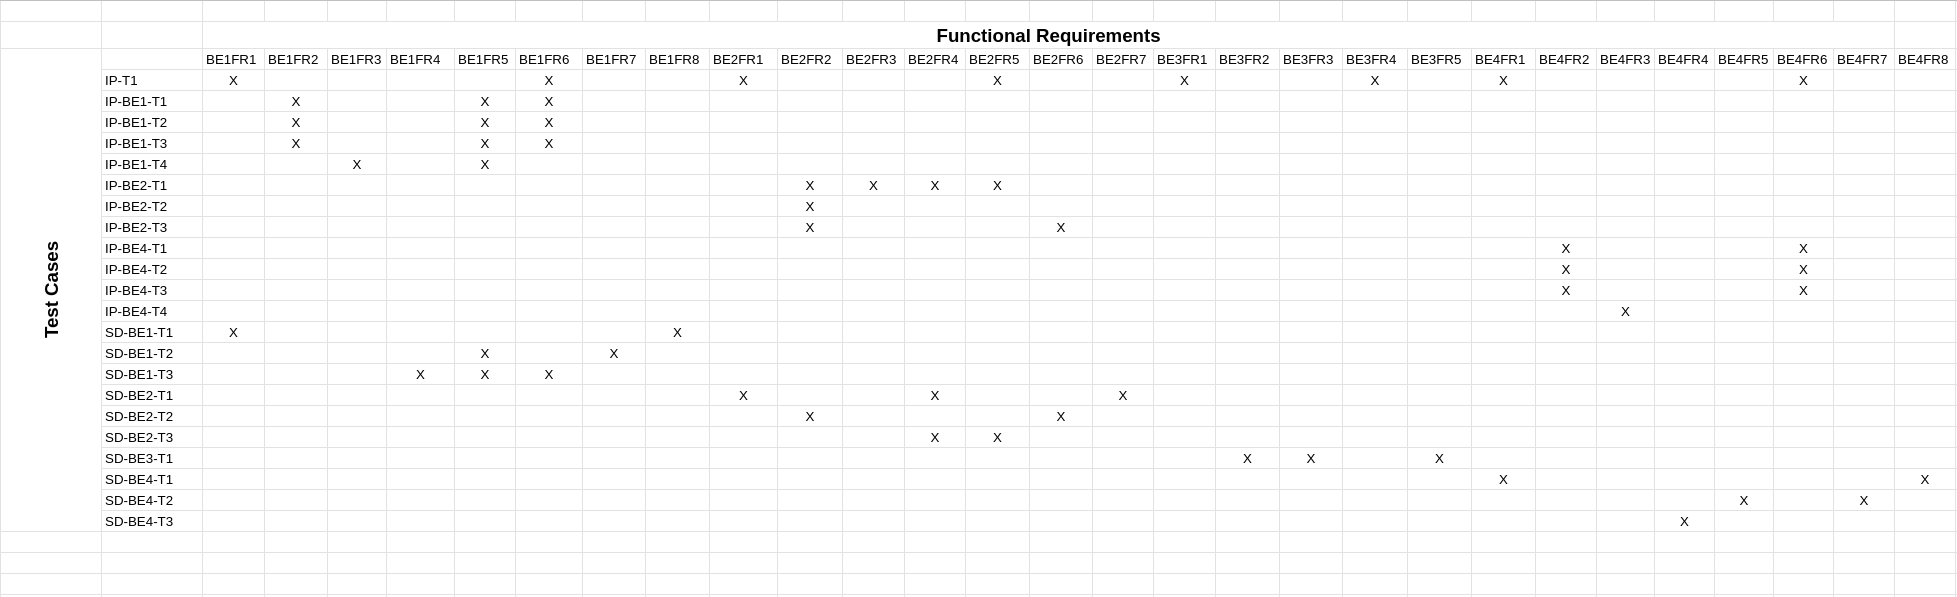
\includegraphics[scale=0.25, angle=90]{FR-1.png}
    \caption{Traceability Matrix for Functional Requirements in BE1 to BE4}
    \label{fig:my_label}
\end{figure}

\begin{figure}[H]
    \centering
    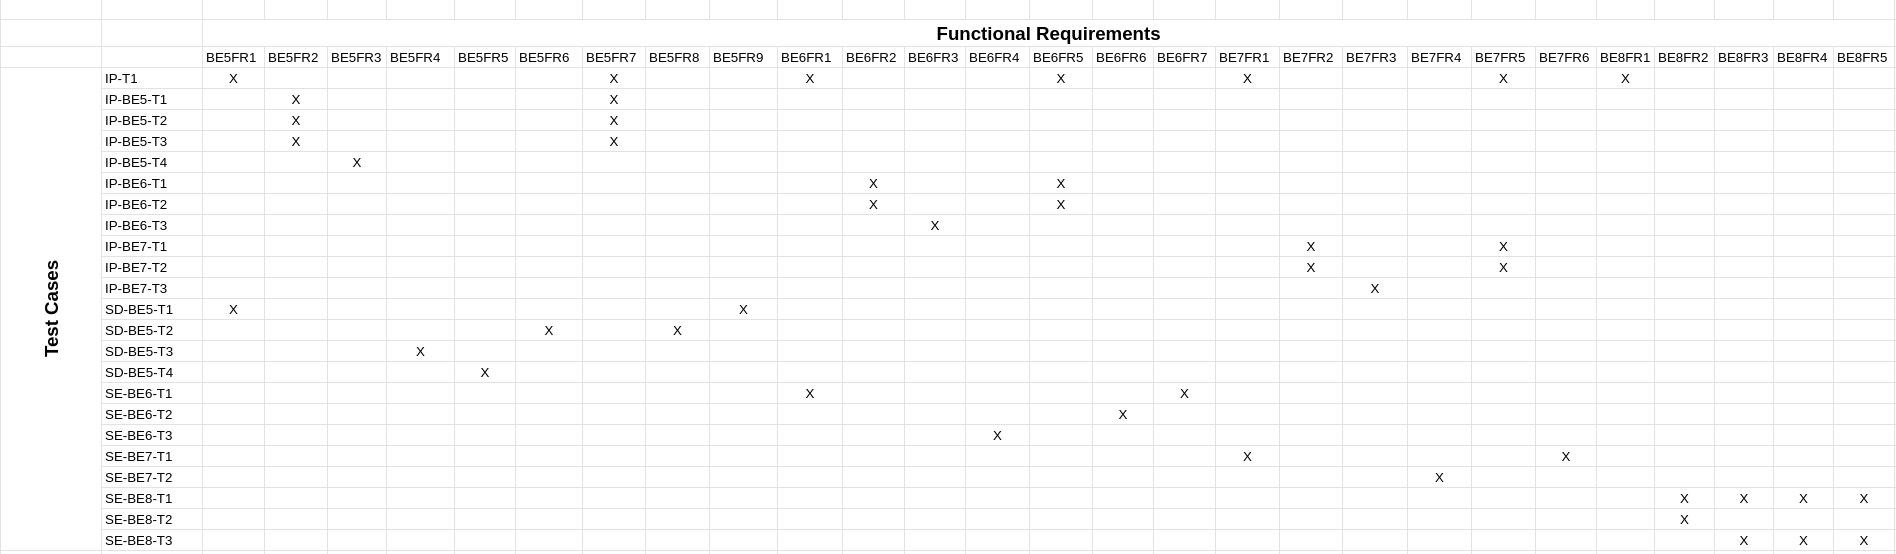
\includegraphics[scale=0.25, angle=90]{FR-2.png}
    \caption{Traceability Matrix for Functional Requirements in BE5 to BE8}
    \label{fig:my_label}
\end{figure}

\begin{figure}[H]
    \centering
    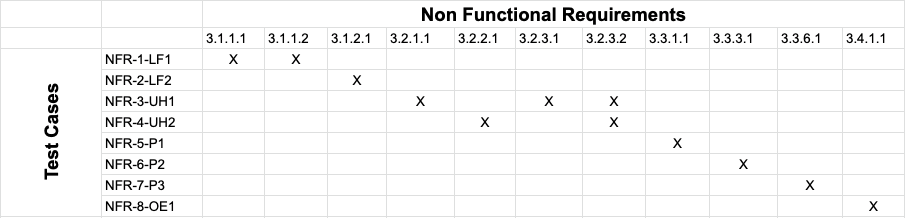
\includegraphics[scale=0.50, angle=90]{NFR.png}
    \caption{Traceability Matrix for Nonfunctional Requirements in NFR-1 to NFR-8}
    \label{fig:my_label}
\end{figure}

\section{Trace To Modules}

\begin{table}[H]
\centering
\begin{tabular}{p{0.2\textwidth} p{0.6\textwidth}}
\toprule
\textbf{AC} & \textbf{Modules}\\
\midrule
\acref{ac1} & \mref{m16}\\
\acref{ac2} & \mref{m13}\\
\acref{ac3} & \mref{m1}\\
\acref{ac4} & \mref{m1}\\
\acref{ac5} & \mref{m3}, \mref{m10}, {\color{red}\mref{m17}}\\
\acref{ac6} & \mref{m13}\\
\acref{ac7} & \mref{m14}\\
\bottomrule
\end{tabular}
\caption{Trace Between Anticipated Changes and Modules}
\label{TblACT}
\end{table}

\end{document}